\subsection{Insertion Sort}

\begin{table}[h]
	\begin{center}
		\begin{tabular} { >{\centering\arraybackslash}m{3cm} | >{\centering\arraybackslash}m{2cm} | >{\centering\arraybackslash}m{2cm} }
			\hline
			\textbf{Language}	& \textbf{Time(s)} & \textbf{Ratio} \\ \hline
			C\#					& 0.078 		& 1:1 \\ \hline
			Java				& 0.131 		& 1:1.7 \\ \hline
			Python				& 12.525 		& 1:160 \\  \hline		
		\end{tabular}
	\end{center}
	\caption{Results from sorting 10'000 elements using Insertion Sort.}
	\label{table:insertion_sort}
\end{table}

Table \ref{table:insertion_sort} illustrates the time it takes for each language to sort 10'000 positive integers in random order. Notice the time differences between Python and the other two languages.

\begin{figure}[h]
	\centering
	\mbox{
		\subfigure[Test results for Insertion Sort in Java and C\#.]{
			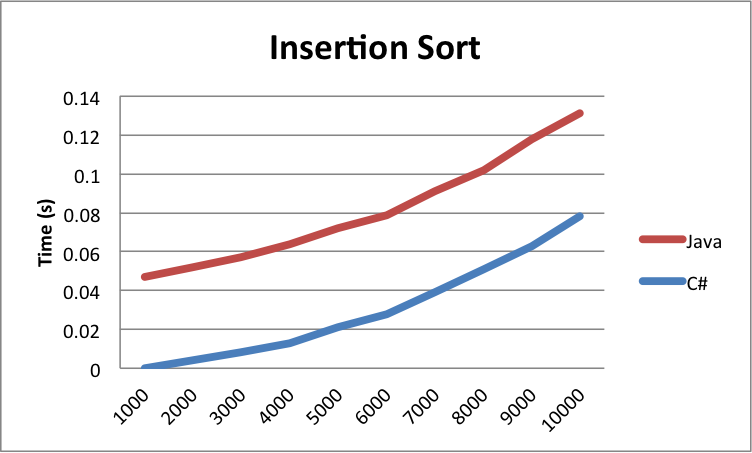
\includegraphics[width=0.48\textwidth]{chapters/media/insertion_sort_csharp_java.png}
			\label{fig:insertion_sort_csharp_java}
		}
		\subfigure[Test results from Insertion Sort in Python.]{
			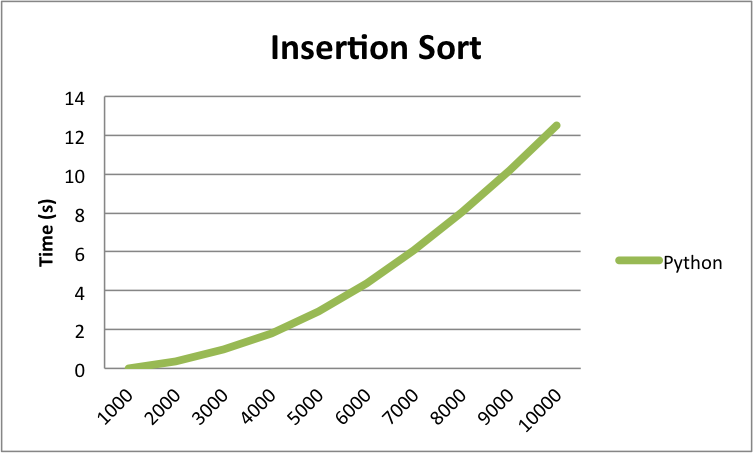
\includegraphics[width=0.48\textwidth]{chapters/media/insertion_sort_python.png}
			\label{fig:insertion_sort_python}
		}
	}
	\caption{Test results for Insertion Sort in C\# and Java to the left and Python to the right.}
	\label{fig:insertion_sort_results}
\end{figure}

Figure \ref{fig:insertion_sort_results} illustrates the relation between the number of positive integers in random order (horizontal-axis) and the time (vertical-axis), the graph looks like the expected quadratic curve since the algorithm runs in $O(n^2)$. Note the time difference on the vertical axis when comparing Figure \ref{fig:insertion_sort_csharp_java} and \ref{fig:insertion_sort_python}.

\begin{figure}[h]
	\centering
	\mbox{
		\subfigure[Java under the .NET Environment and the native environment.]{
			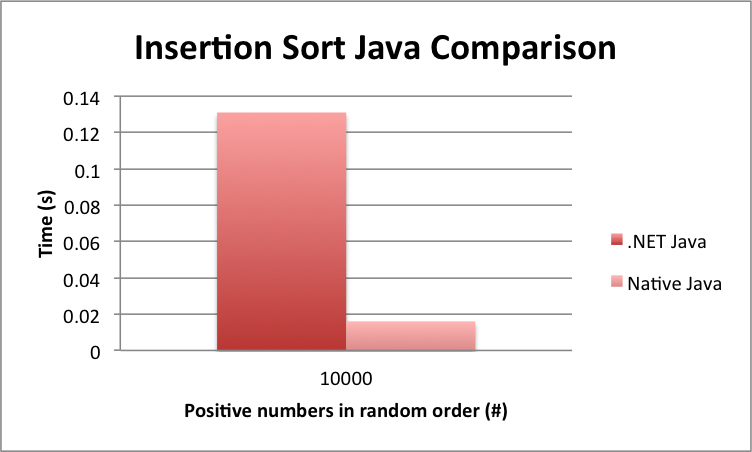
\includegraphics[width=0.48\textwidth]{chapters/media/insertion_sort_native_java.png}
			\label{fig:insertion_sort_native_java}
		}
		\subfigure[Python under the .NET Environment and the native environment.]{
			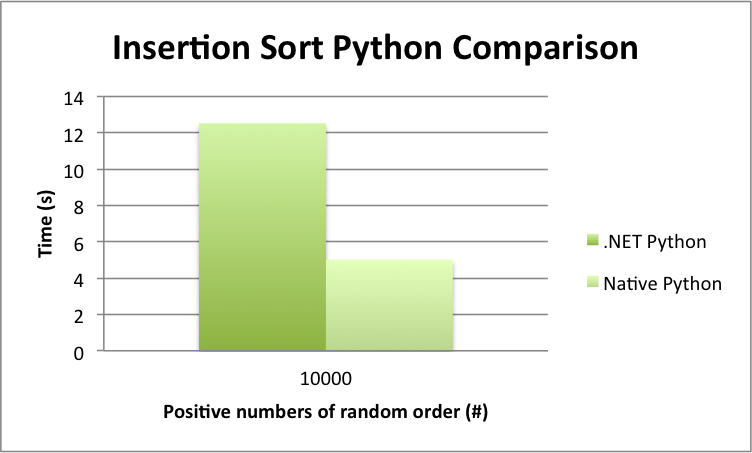
\includegraphics[width=0.48\textwidth]{chapters/media/insertion_sort_native_python.png}
			\label{fig:insertion_sort_native_python}
		}
	}
	\caption{Comparison of running under the .NET Environment and the native environment with Java to the left and Python to the right (using 10'000 elements).}
	\label{fig:insertion_sort_natives}
\end{figure}

Figure \ref{fig:insertion_sort_natives} illustrates the difference in executing code under the .NET environment related to the languages own native environment. Again, note the time difference between the two graphs.

\begin{figure}[h]
	\centering
	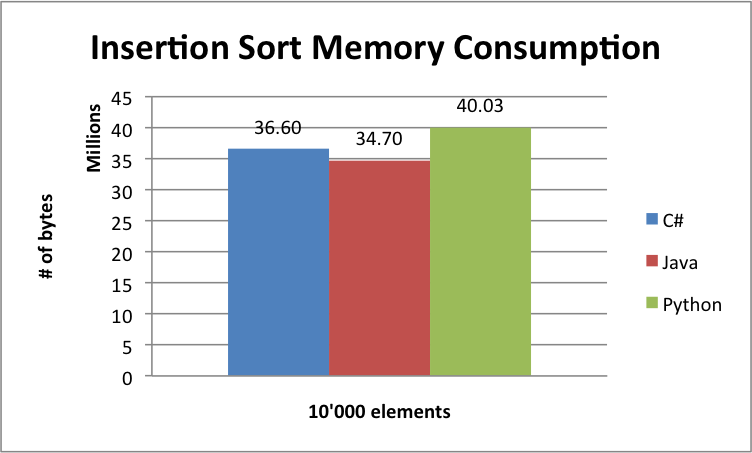
\includegraphics[width=0.6\textwidth]{chapters/media/insertion_sort_memory.png}
	\caption{Comparison of the memory consumption between the three languages.}
	\label{fig:insertion_sort_memory}
\end{figure}

The memory consumption is similar among all languages for Insertion Sort. Python consumed about 10\% - 15\% more with 40 Mb compared with C\# at 36 Mb and Java at 34 Mb (see Figure \ref{fig:insertion_sort_memory}).




















